%%%%%%%%%%%%%%%%%%%%%%%%%%%%%%%%%%%%%%%%%%%%%%%%%%%%%%%%%%%%%%%%%%%%%%%%%%%%%%%%
%%%%%%%%%%%%%%%%%%%%%%%%%%%%%%%%%%%%%%%%%%%%%%%%%%%%%%%%%%%%%%%%%%%%%%%%%%%%%%%%
%%%%%%%%%%%%%%%%%%%%%%%%%%%%%%%%%%%%%%%%%%%%%%%%%%%%%%%%%%%%%%%%%%%%%%%%%%%%%%%%
%%%%%%%%%%%%%%%%%%%%%%%%%%%%%%%%%%%%%%%%%%%%%%%%%%%%%%%%%%%%%%%%%%%%%%%%%%%%%%%%
\chapter{Initiation à Scilab\label{annexe-scilab}}
%%%%%%%%%%%%%%%%%%%%%%%%%%%%%%%%%%%%%%%%%%%%%%%%%%%%%%%%%%%%%%%%%%%%%%%%%%%%%%%%
%%%%%%%%%%%%%%%%%%%%%%%%%%%%%%%%%%%%%%%%%%%%%%%%%%%%%%%%%%%%%%%%%%%%%%%%%%%%%%%%
%%%%%%%%%%%%%%%%%%%%%%%%%%%%%%%%%%%%%%%%%%%%%%%%%%%%%%%%%%%%%%%%%%%%%%%%%%%%%%%%
%%%%%%%%%%%%%%%%%%%%%%%%%%%%%%%%%%%%%%%%%%%%%%%%%%%%%%%%%%%%%%%%%%%%%%%%%%%%%%%%

%%%%%%%%%%%%%%%%%%%%%%%%%%%%%%%%%%%%%%%%%%%%%%%%%%%%%%%%%%%%%%%%%%%%%%%%%%%%%%%%
%%%%%%%%%%%%%%%%%%%%%%%%%%%%%%%%%%%%%%%%%%%%%%%%%%%%%%%%%%%%%%%%%%%%%%%%%%%%%%%%
%%%%%%%%%%%%%%%%%%%%%%%%%%%%%%%%%%%%%%%%%%%%%%%%%%%%%%%%%%%%%%%%%%%%%%%%%%%%%%%%
\section[Présentation générale]
        {Présentation générale 
        (source \href{https://fr.wikipedia.org/wiki/Scilab}{Wikipédia})}
%%%%%%%%%%%%%%%%%%%%%%%%%%%%%%%%%%%%%%%%%%%%%%%%%%%%%%%%%%%%%%%%%%%%%%%%%%%%%%%%
%%%%%%%%%%%%%%%%%%%%%%%%%%%%%%%%%%%%%%%%%%%%%%%%%%%%%%%%%%%%%%%%%%%%%%%%%%%%%%%%
%%%%%%%%%%%%%%%%%%%%%%%%%%%%%%%%%%%%%%%%%%%%%%%%%%%%%%%%%%%%%%%%%%%%%%%%%%%%%%%%
Scilab est un logiciel libre
de calcul numérique fournissant un environnement de
calcul pour des applications scientifiques. 
Il est utilisé pour le traitement 
du signal, l'analyse statistique, 
le traitement d'images, les simulations de 
dynamique des fluides, l'optimisation numérique, et la 
modélisation et simulation de systèmes dynamiques.

La syntaxe et les possibilités offertes par Scilab sont 
similaires à celles de Matlab.

Scilab peut exécuter des instructions en ligne de commande, ainsi que 
des fichiers de commande (scripts) contenant des instructions (format texte). 
On peut exécuter des programmes Fortran ou C à partir de Scilab.
Scilab est complété par un environnement graphique Xcos comparable 
à l'environnement graphique Simulink fourni avec Matlab. 

%\newpage
%%%%%%%%%%%%%%%%%%%%%%%%%%%%%%%%%%%%%%%%%%%%%%%%%%%%%%%%%%%%%%%%%%%%%%%%%%%%%%%%
%%%%%%%%%%%%%%%%%%%%%%%%%%%%%%%%%%%%%%%%%%%%%%%%%%%%%%%%%%%%%%%%%%%%%%%%%%%%%%%%
%%%%%%%%%%%%%%%%%%%%%%%%%%%%%%%%%%%%%%%%%%%%%%%%%%%%%%%%%%%%%%%%%%%%%%%%%%%%%%%%
\section{Syntaxe : console}
%%%%%%%%%%%%%%%%%%%%%%%%%%%%%%%%%%%%%%%%%%%%%%%%%%%%%%%%%%%%%%%%%%%%%%%%%%%%%%%%
%%%%%%%%%%%%%%%%%%%%%%%%%%%%%%%%%%%%%%%%%%%%%%%%%%%%%%%%%%%%%%%%%%%%%%%%%%%%%%%%
%%%%%%%%%%%%%%%%%%%%%%%%%%%%%%%%%%%%%%%%%%%%%%%%%%%%%%%%%%%%%%%%%%%%%%%%%%%%%%%%
Les instructions sont tapées après le prompt \verb?-->?. Le résultat est donné 
sauf si l'instruction se termine par un point-virgule auquel cas le résultat 
est caché. Les variables sont sensibles à la casse. \verb?ans? est la variable 
qui contient le dernier résultat. Un commentaire commence par  \verb?\\?. 
La plupart des opérateurs sont communs avec d'autres langages 
(affectation~\verb?=?, addition~\verb?+?, soustraction~\verb?-?, 
multiplication~\verb?*?, puissance~\verb?** ou ^? ).

%%%%%%%%%%%%%%%%%%%%%%%%%%%%%%%%%%%%%%%%%%%%%%%%%%%%%%%%%%%%%%%%%%%%%%%%%%%%%%%%
\paragraph{Exemples :}
%%%%%%%%%%%%%%%%%%%%%%%%%%%%%%%%%%%%%%%%%%%%%%%%%%%%%%%%%%%%%%%%%%%%%%%%%%%%%%%%
\begin{code}
\begin{verbatim}
-->// ceci n'est pas un commentaire

-->a=2
 a  =
      
    2. 
-->A=3;  \\ le résultat est caché

-->a*A   \\ produit
 ans  =

    6.  
-->ans**2 \\ utilisation de la valeur précédente
 ans  =
  
    36.  
\end{verbatim}
\end{code}

Il existe quelques variables prédéfinies sous Scilab, elles sont appelées à 
l'aide du symbole \og\verb?%?\fg. La liste de ces variables est accessible 
par la fonction \verb?whos -name %?
\begin{code}
\begin{verbatim}
%e    // constante d'Euler
%eps  // précision machine epsilon
%F %f // booléen false 0 
%T %t // booléen True 1 
%pi   // constante pi
%i    // nombre imaginaire
%inf  // infini
%nan  // not-a-number
%s %z // définition de polynômes
\end{verbatim}
\end{code}


Quelques opérateurs logiques : 
\begin{code}
\begin{verbatim}
-->A=0;

-->B=1;

-->A&B    // ET logique
 ans  =
 
  F 

-->A|B    // OU logique
 ans  =
 
  T 

-->~A     // NON logique
 ans  =
 
  T 

-->A==B   // Egalité logique
 ans  =
 
  F

-->A~=B   // Différence logique
 ans  =
 
  T
\end{verbatim}
\end{code}


%%%%%%%%%%%%%%%%%%%%%%%%%%%%%%%%%%%%%%%%%%%%%%%%%%%%%%%%%%%%%%%%%%%%%%%%%%%%%%%%
%%%%%%%%%%%%%%%%%%%%%%%%%%%%%%%%%%%%%%%%%%%%%%%%%%%%%%%%%%%%%%%%%%%%%%%%%%%%%%%%
%%%%%%%%%%%%%%%%%%%%%%%%%%%%%%%%%%%%%%%%%%%%%%%%%%%%%%%%%%%%%%%%%%%%%%%%%%%%%%%%
\section{Polynômes et fractions rationnelles}
%%%%%%%%%%%%%%%%%%%%%%%%%%%%%%%%%%%%%%%%%%%%%%%%%%%%%%%%%%%%%%%%%%%%%%%%%%%%%%%%
%%%%%%%%%%%%%%%%%%%%%%%%%%%%%%%%%%%%%%%%%%%%%%%%%%%%%%%%%%%%%%%%%%%%%%%%%%%%%%%%
%%%%%%%%%%%%%%%%%%%%%%%%%%%%%%%%%%%%%%%%%%%%%%%%%%%%%%%%%%%%%%%%%%%%%%%%%%%%%%%%
En automatique, la définition de la fonction de transfert 
fait intervenir des polynômes et des fractions rationnelles.

La déclaration d'un polynôme se fait à l'aide de deux instructions. 
La première utilise la fonction \verb?poly(0, "p")? qui définit 
\og \verb?p?\fg comme l'indéterminée d'un polynôme. 
La seconde instuction est l'énoncé du polynôme utilisant cette indéterminée. 

%%%%%%%%%%%%%%%%%%%%%%%%%%%%%%%%%%%%%%%%%%%%%%%%%%%%%%%%%%%%%%%%%%%%%%%%%%%%%%%%
\paragraph{Exemple :}
%%%%%%%%%%%%%%%%%%%%%%%%%%%%%%%%%%%%%%%%%%%%%%%%%%%%%%%%%%%%%%%%%%%%%%%%%%%%%%%%

On définit deux polynômes $D(p)=1+2p+3p^2$ et $N(p)=1+p$ de la façon 
suivante :
\begin{code}
\begin{verbatim}
-->p = poly(0, 'p');

-->D=(1+2*p+3*p**2)
 D  =
 
               2  
    1 + 2p + 3p 

-->N=1+p
 N  =
 
    1 + p
\end{verbatim}
\end{code}

La fonction \verb?roots(D)? donne les racines du polynôme $D(p)$ :

\begin{code}
\begin{verbatim}
-->roots(D)
 ans  =
 
  - 0.3333333 + 0.4714045i     // nombre complexe 
  - 0.3333333 - 0.4714045i     // 
-->roots(N)
 ans  =
  
   - 1.
\end{verbatim}
\end{code}

Scilab gère de la même manière les fractions rationnelles :
\begin{code}
\begin{verbatim}
-->H=N/D
 H  =
 
       1 + p      
    -----------   
               2  
    1 + 2p + 3p 
\end{verbatim}
\end{code}

Il est possible d'extraire les numérateurs et dénominateurs de 
$H(p)=N(p)/D(p)$ par les variables \verb?H.num? et \verb?H.den? 
respectivement :
\begin{code}
\begin{verbatim}
-->roots(H.den)               // pôles
 ans  =
 
  - 0.3333333 + 0.4714045i  
  - 0.3333333 - 0.4714045i

-->roots(H.num)               // zéros
 ans  =
 
  - 1.
\end{verbatim}
\end{code}

Il est également possible de définir un polynôme à partir de ces racines 
ou de ces coefficients en appelant seulement la fonction \verb?poly?.

%%%%%%%%%%%%%%%%%%%%%%%%%%%%%%%%%%%%%%%%%%%%%%%%%%%%%%%%%%%%%%%%%%%%%%%%%%%%%%%%
\paragraph{\`A partir de ses racines:}
%%%%%%%%%%%%%%%%%%%%%%%%%%%%%%%%%%%%%%%%%%%%%%%%%%%%%%%%%%%%%%%%%%%%%%%%%%%%%%%%

\begin{code}
\begin{verbatim}
-->poly([1 2],'p')    // polynôme dont les racines sont 1 et 2
 ans  =
 
              2  
    2 - 3p + p 
\end{verbatim}
\end{code}

%%%%%%%%%%%%%%%%%%%%%%%%%%%%%%%%%%%%%%%%%%%%%%%%%%%%%%%%%%%%%%%%%%%%%%%%%%%%%%%%
\paragraph{\`A partir des ses coefficient:}
%%%%%%%%%%%%%%%%%%%%%%%%%%%%%%%%%%%%%%%%%%%%%%%%%%%%%%%%%%%%%%%%%%%%%%%%%%%%%%%%

\begin{code}
\begin{verbatim}
-->poly([1 2],'p','c')    // option 'c' nécessaire
 ans  =
 
    1 + 2p
\end{verbatim}
\end{code}

%%%%%%%%%%%%%%%%%%%%%%%%%%%%%%%%%%%%%%%%%%%%%%%%%%%%%%%%%%%%%%%%%%%%%%%%%%%%%%%%
\paragraph{Remarque:}
%%%%%%%%%%%%%%%%%%%%%%%%%%%%%%%%%%%%%%%%%%%%%%%%%%%%%%%%%%%%%%%%%%%%%%%%%%%%%%%%
Lorsque que l'on écrit \verb?p=poly(0,'p')?, on définit la variable \verb?p? 
comme le polynôme dont la racine est nulle.
\begin{code}
\begin{verbatim}
-->p=poly(0,'p')
 ans  =

    p
\end{verbatim}
\end{code}

Il est également de possible d'utiliser la variable \verb?\%s? qui correspond
à l'instruction \verb?s=poly(0,'s')?.

%%%%%%%%%%%%%%%%%%%%%%%%%%%%%%%%%%%%%%%%%%%%%%%%%%%%%%%%%%%%%%%%%%%%%%%%%%%%%%%%
%%%%%%%%%%%%%%%%%%%%%%%%%%%%%%%%%%%%%%%%%%%%%%%%%%%%%%%%%%%%%%%%%%%%%%%%%%%%%%%%
%%%%%%%%%%%%%%%%%%%%%%%%%%%%%%%%%%%%%%%%%%%%%%%%%%%%%%%%%%%%%%%%%%%%%%%%%%%%%%%%
\section{Vecteurs et matrices}
%%%%%%%%%%%%%%%%%%%%%%%%%%%%%%%%%%%%%%%%%%%%%%%%%%%%%%%%%%%%%%%%%%%%%%%%%%%%%%%%
%%%%%%%%%%%%%%%%%%%%%%%%%%%%%%%%%%%%%%%%%%%%%%%%%%%%%%%%%%%%%%%%%%%%%%%%%%%%%%%%
%%%%%%%%%%%%%%%%%%%%%%%%%%%%%%%%%%%%%%%%%%%%%%%%%%%%%%%%%%%%%%%%%%%%%%%%%%%%%%%%

%Scilab est adapté au calcul vectoriel/ matriciel numérique. 

Pour définir un vecteur ligne :
\begin{code}
\begin{verbatim}
--> v=[1,2,3]
 v  =
 
    1.    2.    3. 

-->v=1:3
 v  =
 
    1.    2.    3.

-->v=1:0.5:4              // a:incr:b
 v  =                     // liste allant de a à b par incrément 
                          // de incr
 
    1.    1.5    2.    2.5    3.    3.5    4.
\end{verbatim}
\end{code}

Pour définir un vecteur colonne :
\begin{code}
\begin{verbatim}
--> v=[1;2;3]
 v  =
 
    1.    
    2.
    3. 
\end{verbatim}
\end{code}

Nous combinons les deux syntaxes précédentes pour définir une matrice : 
\begin{code}
\begin{verbatim}
--> m=[1 2; 3 4 ; 5 6]
 m  =
 
    1.    2.  
    3.    4.  
    5.    6.  
\end{verbatim}
\end{code}

Le vecteur ou la liste nul est simplement déclaré par :
\begin{code}
\begin{verbatim}
-->liste=[];
\end{verbatim}
\end{code}

Les parenthèses permettent d'accéder aux élément d'une matrice et le 
symbole \og\verb?:?\fg permet d'accéder à toute ou une partie d'une 
ligne ou d'une colonne
\begin{code}
\begin{verbatim}
-->v(1)
 ans  =
 
    1.  

-->m(2,1)
 ans  =
 
    3.  
--> // accéder à une ligne entière
 
-->m(1,:)
 ans  =
   
     1.    2. 
\end{verbatim}
\end{code}

%\newpage
Pour concaténer deux vecteurs ou matrices :
\begin{code}
\begin{verbatim}
-->u=[1,2,3];
 
-->v=[4,5,6];
 
-->w=[v,u]
 w  =
 
    4.    5.    6.    1.    2.    3.

-->m1=[1 2; 3 4 ; 5 6]
 
-->m2=[1 2; 3 4 ; 5 6]
 
-->m3=[m1,m2]
 m3  =
 
    1.    2.    1.    2.  
    3.    4.    3.    4.  
    5.    6.    5.    6. 
\end{verbatim}
\end{code}
\paragraph{Fonctions pour construire des vecteurs et matrices élémentaires}
On utilisera la fonction ones pour construire un vecteur ou une matrice remplie 
de 1.
Exemple pour construire un vecteur de 10 composantes de valeurs 1 :
\begin{code}
\begin{verbatim}
--> ones(1,10)
 ans  =

    1.   1.   1.   1.   1.   1.   1.   1.   1.   1.

\end{verbatim}
\end{code}
pour une matrice 3x3 :
\begin{code}
\begin{verbatim}
--> ones(3,3)
 ans  =

    1.   1.   1.
    1.   1.   1.
    1.   1.   1.
\end{verbatim}
\end{code}

Les fonctions \verb?zeros? et \verb?rand? fonctionnent sur le même principe 
pour construire respectivement des vecteurs et matrices de zéros ou de nombres aléatoires.

Les fonctions \verb?linspace? et \verb?logspace? permettent de construire respectivement 
des vecteurs de valeurs linairement et logarithmiquement équidistantes.  

Par exemple l'instruction suivante construit un vecteur de 9 éléments équidistants (de 0.5) 
dont les valeures sont comprises entre 1 et 5 :
\begin{code}
\begin{verbatim}
--> linspace(1,5,9)
 ans  =

    1.   1.5   2.   2.5   3.   3.5   4.   4.5   5.
\end{verbatim}
\end{code}
et l'exemple suivant, correspond à un vecteur de 5 éléments dont les valeurs sont logarithmiquement
équidistantes (10) entre 10$^1$ et 10$^5$:
\begin{code}
\begin{verbatim}
--> logspace(1,5,5)
 ans  =

    10.   100.   1000.   10000.   100000.

\end{verbatim}
\end{code}

%%%%%%%%%%%%%%%%%%%%%%%%%%%%%%%%%%%%%%%%%%%%%%%%%%%%%%%%%%%%%%%%%%%%%%%%%%%%%%%%
\paragraph{Opération élément par élément}
%%%%%%%%%%%%%%%%%%%%%%%%%%%%%%%%%%%%%%%%%%%%%%%%%%%%%%%%%%%%%%%%%%%%%%%%%%%%%%%%

Les opérateurs mathématiques de bases peuvent être utilisés 
sur les vecteur et matrices mais doivent respecter une certaine 
cohérence des dimensions des objets de chaque coté de l'opérateur. 
Notamment, les opérations \verb?*? et \verb?/? sont des opérations 
matricielles. Pour faire des opérations élément par élément,
on fera précéder le signe opératoire d'un point : \verb?.*? \verb?./?.

Exemple :
\begin{code}
\begin{verbatim}
// définition de l'indéterminée du polynôme
-->p = poly(0, 'p');

//définition d'un vecteur de numérateurs
-->num=[1 10 20];

//définition d'un vecteur de dénominateurs
-->den=[p*(p+1) p*(p+10) p*(p+20) ];

//définition d'un vecteur de fonctions de transfert
-->H=num ./ den
 H  =
 
      1         10          20      
    -----     ------      ------    
         2           2           2  
    p + p     10p + p     20p + p   
\end{verbatim}
\end{code}

Scilab a été conçu pour le calcul matriciel et numérique. 
Il existe de nombreuses opérations spécifiques aux matrices et à la 
résolution numériques que nous ne traiterons pas dans ce document.

Pour accéder à l'aide en ligne, cliquez sur \verb/ ? >Aide Scilab/ 
dans la barre de menus, ou tapez   dans la console :
\begin{code}
\begin{verbatim}
-->help <fonction>
\end{verbatim}
\end{code}

%%%%%%%%%%%%%%%%%%%%%%%%%%%%%%%%%%%%%%%%%%%%%%%%%%%%%%%%%%%%%%%%%%%%%%%%%%%%%%%%
%%%%%%%%%%%%%%%%%%%%%%%%%%%%%%%%%%%%%%%%%%%%%%%%%%%%%%%%%%%%%%%%%%%%%%%%%%%%%%%%
%%%%%%%%%%%%%%%%%%%%%%%%%%%%%%%%%%%%%%%%%%%%%%%%%%%%%%%%%%%%%%%%%%%%%%%%%%%%%%%%
\section{Tracer de figures}
%%%%%%%%%%%%%%%%%%%%%%%%%%%%%%%%%%%%%%%%%%%%%%%%%%%%%%%%%%%%%%%%%%%%%%%%%%%%%%%%
%%%%%%%%%%%%%%%%%%%%%%%%%%%%%%%%%%%%%%%%%%%%%%%%%%%%%%%%%%%%%%%%%%%%%%%%%%%%%%%%
%%%%%%%%%%%%%%%%%%%%%%%%%%%%%%%%%%%%%%%%%%%%%%%%%%%%%%%%%%%%%%%%%%%%%%%%%%%%%%%%
On utilisera les fonctions \verb?scf? et \verb?clf?  pour respectivement
créer une nouvelle fenêtre graphique et éffacer le contenu d'une fenêtre 
graphique.

%%%%%%%%%%%%%%%%%%%%%%%%%%%%%%%%%%%%%%%%%%%%%%%%%%%%%%%%%%%%%%%%%%%%%%%%%%%%%%%%
\paragraph{Exemple : plot de deux fenêtres (sinus/cosinus)}
%%%%%%%%%%%%%%%%%%%%%%%%%%%%%%%%%%%%%%%%%%%%%%%%%%%%%%%%%%%%%%%%%%%%%%%%%%%%%%%%
Le code suivant permet de tracer les fonctions sinus et cosinus sur deux fenetres
distinctes. 

\begin{code}
\begin{verbatim}
scf(0);clf(0); // création d'une première fenêtre
t=0.0:0.05:10; 
plot(t,sin(t),'r')
legend('$s_1(t)$')
xlabel("$t$","fontsize",4);
ylabel("$s_1(t)$","fontsize",4);
title('fonction sinus',"fontsize",4);

scf(1);clf(1); // création d'une seconde fenêtre    
t=0.0:0.05:10;
plot(t,cos(t),'r')
legend('$s_2(t)$')
xlabel("$t$","fontsize",4);
ylabel("$s_2(t)$","fontsize",4);
title('fonction cosinus',"fontsize",4);  
\end{verbatim}
\end{code}

\begin{figure}[!ht]
    \centering
    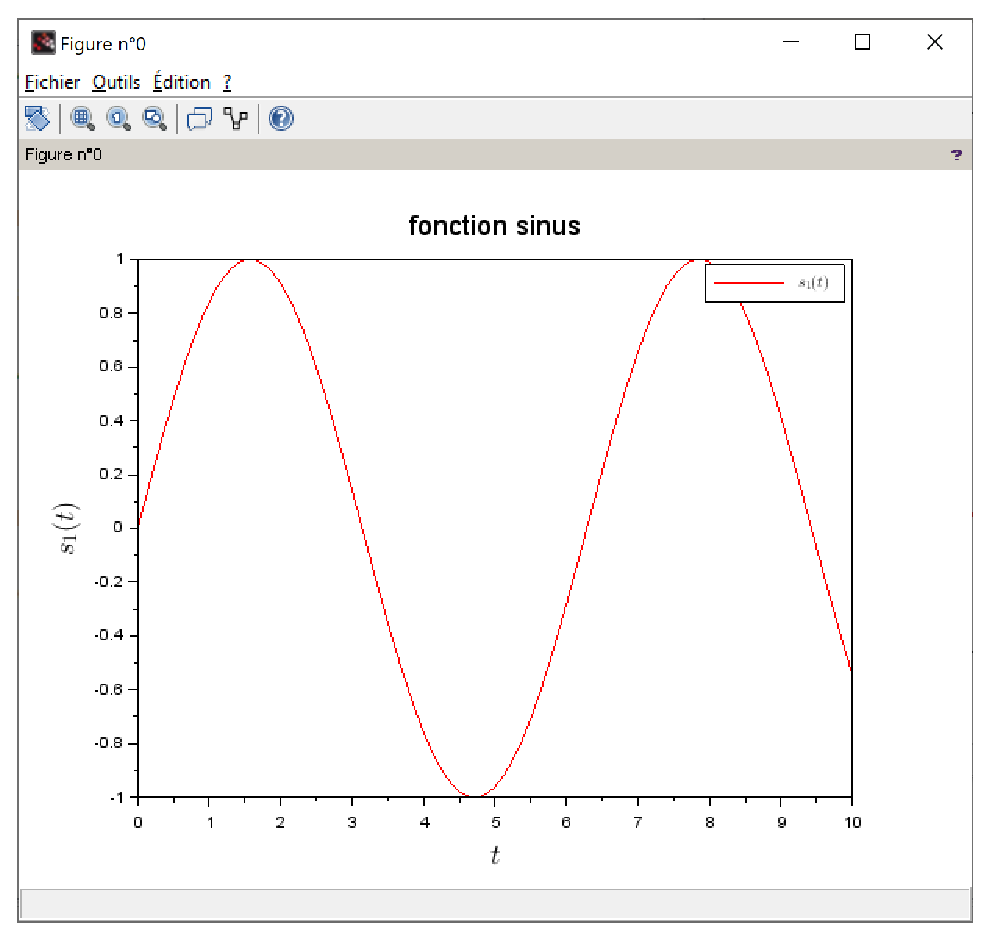
\includegraphics[width=0.8\textwidth]{fig/capture_SCILAB.eps}
    \caption{Capture d'écran de la fenêtre graphique générée par SCILAB.\label{fig-capture-SCILAB}}
\end{figure}

La figure~\cref{fig-capture-SCILAB} présente une capture d'écran 
d'une des fenêtres générées par SCILAB.
          
Les textes des légendes, titre des axes acceptent la syntaxe~\LaTeX.
Il existe de nombreuses commandes pour modifier l'apparence
d'une figure, de ces axes et pour pouvoir la sauvegarder
dans différents formats (vectorielle ou matricielle).
Nous renvoyons au lecteur à la documentation de Scilab pour
cet aspect. Il est également possible d'éditer une image en accédant
au menu de la fenêtre graphique après l'avoir générée.


%%%%%%%%%%%%%%%%%%%%%%%%%%%%%%%%%%%%%%%%%%%%%%%%%%%%%%%%%%%%%%%%%%%%%%%%%%%%%%%%
%%%%%%%%%%%%%%%%%%%%%%%%%%%%%%%%%%%%%%%%%%%%%%%%%%%%%%%%%%%%%%%%%%%%%%%%%%%%%%%%
%%%%%%%%%%%%%%%%%%%%%%%%%%%%%%%%%%%%%%%%%%%%%%%%%%%%%%%%%%%%%%%%%%%%%%%%%%%%%%%%
%%%%%%%%%%%%%%%%%%%%%%%%%%%%%%%%%%%%%%%%%%%%%%%%%%%%%%%%%%%%%%%%%%%%%%%%%%%%%%%%
\section[Programmation]
        {Programmation (source 
        \href{https://fr.wikibooks.org/wiki/Découvrir_Scilab}{Wikibooks}) }
%%%%%%%%%%%%%%%%%%%%%%%%%%%%%%%%%%%%%%%%%%%%%%%%%%%%%%%%%%%%%%%%%%%%%%%%%%%%%%%%
%%%%%%%%%%%%%%%%%%%%%%%%%%%%%%%%%%%%%%%%%%%%%%%%%%%%%%%%%%%%%%%%%%%%%%%%%%%%%%%%
%%%%%%%%%%%%%%%%%%%%%%%%%%%%%%%%%%%%%%%%%%%%%%%%%%%%%%%%%%%%%%%%%%%%%%%%%%%%%%%%
%%%%%%%%%%%%%%%%%%%%%%%%%%%%%%%%%%%%%%%%%%%%%%%%%%%%%%%%%%%%%%%%%%%%%%%%%%%%%%%%

Scilab est également un langage de programmation, il accepte un certain nombre 
d'instructions autres que mathématiques, permettant la formulation et 
l'exécution d'algorithmes : \verb?for, while, if, do, do, case?\ldots ou 
définition de fonction.

L'écriture de programmes se fait idéalement avec l'éditeur de 
texte SciNotes; celui-ci met en exergue les instructions en couleurs, 
les parenthésages (correspondance entre les paires de parenthèses 
et de crochets), et surligne les lignes continuées avec un fond jaune. 
On peut aussi utiliser un autre éditeur de texte en sauvegardant le fichier 
avec l'extension \verb?.sce? ou \verb?.sci?. Lorsque l'environnement le permet,
on peut faire du copier-coller depuis l'éditeur de texte externe vers SciNotes 
ou bien l'éditeur de ligne de commande.

%%%%%%%%%%%%%%%%%%%%%%%%%%%%%%%%%%%%%%%%%%%%%%%%%%%%%%%%%%%%%%%%%%%%%%%%%%%%%%%%
\paragraph{Syntaxe d'une fonction :}
%%%%%%%%%%%%%%%%%%%%%%%%%%%%%%%%%%%%%%%%%%%%%%%%%%%%%%%%%%%%%%%%%%%%%%%%%%%%%%%%

La fonction doit commencer par le mot réservé \verb?function? et finir par 
\verb?endfunction? sous la forme :
\begin{code}
\begin{verbatim}
function [out1,out2,...,outN]=nomfonction(in1,in2,...,inP)

  // out1,out2,...,outN sont les variables de sortie
  // in1,in2,...,inP variables d entree
          
<instructions>
endfunction
\end{verbatim}
\end{code}

Une façon usuelle de définir des fonctions est de mettre 
celles-ci dans un fichier à extension \verb?.sci?. 
Il faut alors la charger avec la fonction \verb?exec()?.
Pour exécuter une fonction, il suffit de l'appeler en passant les 
arguments nécessaires.

%%%%%%%%%%%%%%%%%%%%%%%%%%%%%%%%%%%%%%%%%%%%%%%%%%%%%%%%%%%%%%%%%%%%%%%%%%%%%%%%
\paragraph{Exemple d'une réponse temporelle analytique}
%%%%%%%%%%%%%%%%%%%%%%%%%%%%%%%%%%%%%%%%%%%%%%%%%%%%%%%%%%%%%%%%%%%%%%%%%%%%%%%%
Nous souhaitons tracer la réponse temporelle d'un système linéaire dont la
forme analytique est déterminée et de la forme :
$$
s(t)=\dfrac{1}{2}-e^{-t}-\dfrac{3}{2}e^{-2t}
$$
On écrira la fonction de la façon suivante :
\begin{code}
\begin{verbatim}
function u=s(t)
    u=0.5-exp(-t)+1.5*exp(-2*t)
endfunction
\end{verbatim}
\end{code}

On peut maintenant l'appeler avec un arguments sous la forme de vecteurs. 
\begin{code}
\begin{verbatim}
t=0:0.1:10
plot2d(t,s(t),style=3)
\end{verbatim}
\end{code}
La fonction renvoie un vecteur de même taille que le vecteur \verb?t?.

\begin{center}
    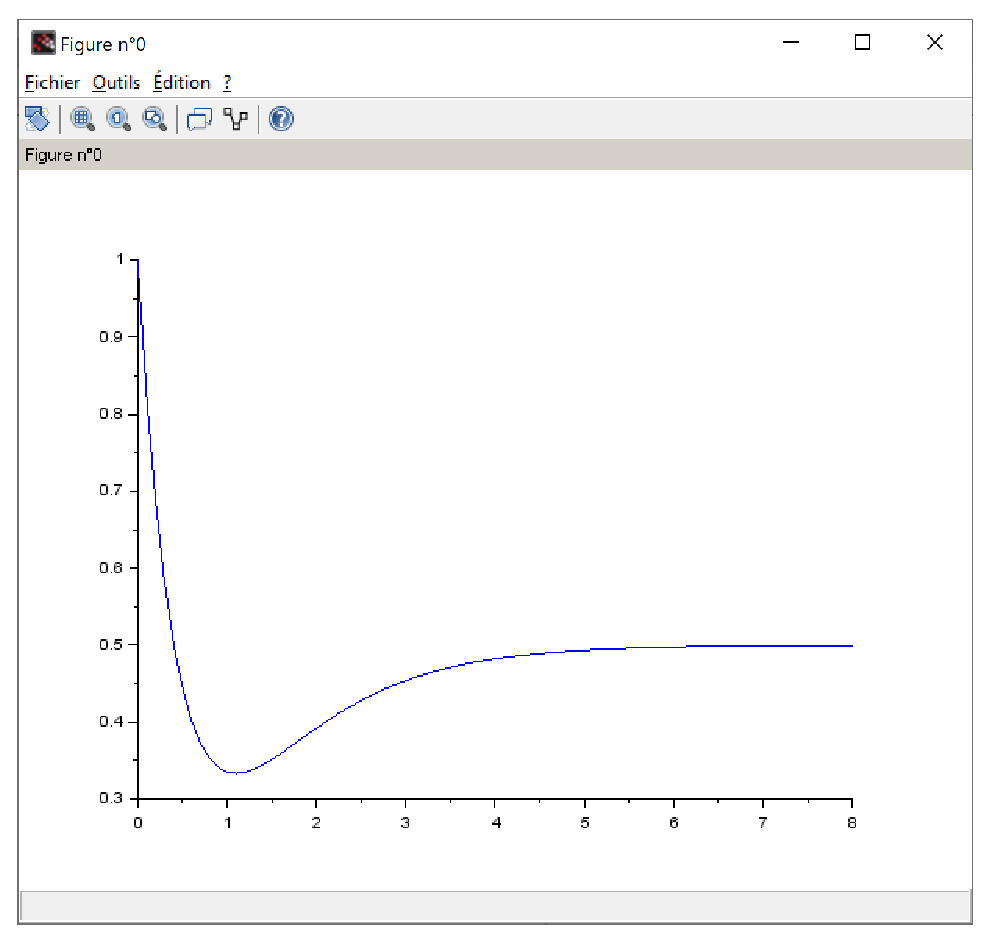
\includegraphics[width=0.5\textwidth]{fig/capture_SCILAB-fonction.eps}
\end{center}

\newpage
%%%%%%%%%%%%%%%%%%%%%%%%%%%%%%%%%%%%%%%%%%%%%%%%%%%%%%%%%%%%%%%%%%%%%%%%%%%%%%%%
%%%%%%%%%%%%%%%%%%%%%%%%%%%%%%%%%%%%%%%%%%%%%%%%%%%%%%%%%%%%%%%%%%%%%%%%%%%%%%%%
%%%%%%%%%%%%%%%%%%%%%%%%%%%%%%%%%%%%%%%%%%%%%%%%%%%%%%%%%%%%%%%%%%%%%%%%%%%%%%%%
\section{\emph{{\scshape SLCI}}~avec Scilab}
%%%%%%%%%%%%%%%%%%%%%%%%%%%%%%%%%%%%%%%%%%%%%%%%%%%%%%%%%%%%%%%%%%%%%%%%%%%%%%%%
%%%%%%%%%%%%%%%%%%%%%%%%%%%%%%%%%%%%%%%%%%%%%%%%%%%%%%%%%%%%%%%%%%%%%%%%%%%%%%%%
%%%%%%%%%%%%%%%%%%%%%%%%%%%%%%%%%%%%%%%%%%%%%%%%%%%%%%%%%%%%%%%%%%%%%%%%%%%%%%%%

Scilab permet de réaliser des études avancées des systèmes linéaires continus 
et invariants.

%%%%%%%%%%%%%%%%%%%%%%%%%%%%%%%%%%%%%%%%%%%%%%%%%%%%%%%%%%%%%%%%%%%%%%%%%%%%%%%%
%%%%%%%%%%%%%%%%%%%%%%%%%%%%%%%%%%%%%%%%%%%%%%%%%%%%%%%%%%%%%%%%%%%%%%%%%%%%%%%%
\subsection{Définition d'un système linéaire}
%%%%%%%%%%%%%%%%%%%%%%%%%%%%%%%%%%%%%%%%%%%%%%%%%%%%%%%%%%%%%%%%%%%%%%%%%%%%%%%%
%%%%%%%%%%%%%%%%%%%%%%%%%%%%%%%%%%%%%%%%%%%%%%%%%%%%%%%%%%%%%%%%%%%%%%%%%%%%%%%%
La définition d'un système linéaire continu se fait avec la fonction 
\verb?syslin?. 

\begin{doc}
%%%%%%%%%%%%%%%%%%%%%%%%%%%%%%%%%%%%%%%%%%%%%%%%%%%%%%%%%%%%%%%%%%%%%%%%%%%%%%%%
\paragraph{Fonction syslin (extrait de la doc officiel: help syslin )}
%%%%%%%%%%%%%%%%%%%%%%%%%%%%%%%%%%%%%%%%%%%%%%%%%%%%%%%%%%%%%%%%%%%%%%%%%%%%%%%%
    \begin{itemize}
        \item Syntaxe :
        \begin{code}
\begin{verbatim}
sl=syslin(dom,N,D)
sl=syslin(dom,H)
\end{verbatim}
        \end{code}
        \item Paramètres :
            \begin{itemize}
                \item \verb?dom? : chaîne de caractères \verb?('c','d')?, 
                      ou \verb?[]? ou un scalaire.
                \item \verb?N,D? : matrices polynomiales
                \item \verb?H?   : matrice rationnelle
                \item \verb?sl?  : tlist (liste de type "\verb?syslin?") 
                      représentant le système dynamique
            \end{itemize}
        \item Description : 
            \begin{itemize}
                \item \verb?syslin? définit un système dynamique linéaire en 
                      tant que liste typée, et vérifie la consistance des 
                      données.
                \item \verb?dom? spécifie le domaine temporel :
                      \verb?dom='c'? pour un système à temps continu, 
                      \verb?dom='d'? pour un système à temps discret, 
                      \verb?n? pour un système échantillonné à la période n 
                      (en secondes), 
                      \verb?dom=[]? si le domaine temporel n'est pas défini
            \end{itemize}
    \end{itemize}
\end{doc}

\paragraph{Exemple d'utilisation}
Pour définir un système linéaire du premier ordre de fonction de transfert
$$
H(p)=\dfrac{K}{1+\tau p}
$$
à l'aide de la fonction \verb?syslin? il existe deux syntaxes, soit en utilisant 
la fraction rationnelle directement \verb?syslin("c",ft)?:
\begin{code}
\begin{verbatim}
// ======================================
//  Définir un système du premier ordre
// ======================================
p=%s                   // indéterminée du polynôme
K=1,tau=1;             // paramètres du système

H=K/(1+tau*p);         // fonction de tranfert

PO=syslin('c',H)       // définition du SLCI PO:PremierOrdre
\end{verbatim}
\end{code}
ou en définisant le numérateur et dénominateur séparément (c.-à-d \verb?syslin("c",num,den)?)
\begin{code}
\begin{verbatim}
p=%s
K=1,tau=1;                // paramètres du système

PO=syslin('c',K,1+tau*p)  // définition du SLCI PO:PremierOrdre
\end{verbatim}
\end{code}

Il faut noter que les paramètres de la fonction de transfert sont affectés de valeurs
numériques. En effet, SCILAB ne peut pas traiter des variables formelles mais uniquement
des variables \og numériques\fg.
%\newpage

%%%%%%%%%%%%%%%%%%%%%%%%%%%%%%%%%%%%%%%%%%%%%%%%%%%%%%%%%%%%%%%%%%%%%%%%%%%%%%%%
%%%%%%%%%%%%%%%%%%%%%%%%%%%%%%%%%%%%%%%%%%%%%%%%%%%%%%%%%%%%%%%%%%%%%%%%%%%%%%%%
\subsection{Simulation temporelle d'un système linéaire}
%%%%%%%%%%%%%%%%%%%%%%%%%%%%%%%%%%%%%%%%%%%%%%%%%%%%%%%%%%%%%%%%%%%%%%%%%%%%%%%%
%%%%%%%%%%%%%%%%%%%%%%%%%%%%%%%%%%%%%%%%%%%%%%%%%%%%%%%%%%%%%%%%%%%%%%%%%%%%%%%%
Pour simuler la réponse temporelle d'un système linéaire on utilisera la fonction 
\verb?csim?.

\begin{doc}
%%%%%%%%%%%%%%%%%%%%%%%%%%%%%%%%%%%%%%%%%%%%%%%%%%%%%%%%%%%%%%%%%%%%%%%%%%%%%%%%
\paragraph{Fonction csim (extrait de la doc officiel (en anglais): help csim )}
%%%%%%%%%%%%%%%%%%%%%%%%%%%%%%%%%%%%%%%%%%%%%%%%%%%%%%%%%%%%%%%%%%%%%%%%%%%%%%%%
\begin{itemize}
    \item Syntax :
    \begin{code}
\begin{verbatim}
[y [,x]]=csim(u,t,sl,[x0 [,tol]])
\end{verbatim}
    \end{code}
    \item Parameters :
    \begin{itemize}
        \item \verb?u?  function, list or string (control)
        \item \verb?t?  real vector specifying times with, \verb?t(1)? is the 
              initial time \verb?(x0=x(t(1)))?.
        \item \verb?sl? syslin list (SIMO linear system) in continuous time.
        \item \verb?y?  a matrix such that \verb?y=[y(t(i)], i=1,..,n?
        \item \verb?x?  a matrix such that \verb?x=[x(t(i)], i=1,..,n?
        \item \verb?tol? a 2 vector \verb?[atol rtol]? defining absolute and 
              relative tolerances for \verb?ode? solver
    \end{itemize}

    \item Description :

    \begin{itemize} 
        \item \verb?csim? simulation of the controlled linear system \verb?sl?.
              \verb?sl? is assumed to be a continuous-time system represented 
              by a \verb?syslin? list.
        \item \verb?u?  is the control and \verb?x0? the initial state.
        \item \verb?y?  is the output and \verb?x? the state.
    \end{itemize}

    The control can be:
    \begin{itemize}
        \item a function : \verb?[inputs]=u(t)?
        \item a list : \verb?list(ut,parameter1,....,parametern)? such that:
              \verb?inputs=ut(t,parameter1,....,parametern)? 
    (\verb?ut? is a function)
        \item the string \verb?"impuls"? for impulse response calculation 
              (here \verb?sl? must have a single input and \verb?x0=0?). 
              For systems with direct feedthrough, the infinite pulse at 
              \verb?t=0? is ignored.
        \item the string \verb?"step"? for step response calculation (here 
              \verb?sl? must have a single input and \verb?x0=0?)
        \item a vector giving the values of \verb?u? corresponding to each 
              \verb?t? value.
\end{itemize}
\end{itemize}
\end{doc}

\paragraph{Exemple d'utilisation}

Pour simuler la réponse impulsionnelle on utilisera la chaîne de caractères 
\verb?'impuls'? (ou les premiers caractères de cette chaîne). 

Il faut également définir le vecteur temps qui imposera la 
taille du vecteur de sortie. Le troisième argument est un système linéaire
définit par la fonction \verb?syslin? présentée précedemment. 
\begin{code}
\begin{verbatim}
t=0.0:0.05:20;              // définition du vecteur 
                            // de temps
// ----------------------
// réponse impulsionnelle
// ----------------------
e1='imp'                    // 'imp' : impulsion de Dirac
s1=csim(e1,t,PO)            // réponse impulsionnelle du sl PO
                            // pour tous les points du vecteur t.

\end{verbatim}
\end{code}
Pour la réponse indicielle, on utilisera la chaîne de caractères \verb?'step'?.
\begin{code}
\begin{verbatim}
t=0.0:0.05:20;              // définition du vecteur 
                            // de temps
// ----------------------
// réponse indicielle 
// ----------------------
e2='step'                   // 'step' : échélon unitaire.
s2=csim(e2,t,PO)            // réponse impulsionnelle du sl PO
                            // pour tous les points du vecteur t.

\end{verbatim}
\end{code}
Pour toute autre fonction, on donnera le vecteur de la fonction explicitement. 
Par exemple pour la réponse à une rampe unitaire on donnera simplement 
le vecteur \verb?t?. \`A noter que pour la réponse indicielle, nous aurions pu utiliser
la fonction \verb?ones? :

\begin{code}
\begin{verbatim}
step=ones(size(t)(1),size(t)(2))
s1=csim(step,t,PO)
\end{verbatim}
\end{code}

On notera que l'on utilise ici la fonction \verb?size()? pour assurer que le vecteur 
de la sollicitation est de même taille que le vecteur \verb?t?. 

\paragraph{Approximation de l'impulsion de Dirac}

Il est possible d'approximée l'impulsion de Dirac par un vecteur dont
les valeurs sont toutes nulles sauf pour sa première composante. 
L'amplitude du \og pic\fg dépendra de l'écart entre deux valeurs du vecteur temps $\Delta t$. 
Les instructions suivantes permettent de verifier cette approximation :

\begin{code}
    \begin{verbatim}
s=%s
//définition d'une fonction de transfert du premier ordre
H=syslin('c',1,1+s+s^2)

t=0:0.001:16
// simulation exacte de la réponse impulsionnelle
exact=csim('imp',t,H)

//approximation de l'impulsion de Dirac
impuls=zeros(size(t)(1),size(t)(2))
impuls(1)=2/(t(2)-t(1))  // "amplitude" de l'impulsion 2/Dt  
//simulation approximée de la réponse impulsionnelle
approx=csim(impuls,t,H)

clf(0)
plot2d(t,[exact' approx'],[1 2])
\end{verbatim}
\end{code}

Cette approximation est d'autant meilleure que l'intervalle $\Delta t$ est petit 
(autrement dit que le nombre de points du vecteur \verb?t?, pour un 
intervalle donnée est grand). On utilisera cette approximation avec prudence.

%%%%%%%%%%%%%%%%%%%%%%%%%%%%%%%%%%%%%%%%%%%%%%%%%%%%%%%%%%%%%%%%%%%%%%%%%%%%%%%%
%%%%%%%%%%%%%%%%%%%%%%%%%%%%%%%%%%%%%%%%%%%%%%%%%%%%%%%%%%%%%%%%%%%%%%%%%%%%%%%%
\subsection{Système du premier ordre}
%%%%%%%%%%%%%%%%%%%%%%%%%%%%%%%%%%%%%%%%%%%%%%%%%%%%%%%%%%%%%%%%%%%%%%%%%%%%%%%%
%%%%%%%%%%%%%%%%%%%%%%%%%%%%%%%%%%%%%%%%%%%%%%%%%%%%%%%%%%%%%%%%%%%%%%%%%%%%%%%%
Soit, un système du premier ordre définit par la fonction de transfert : 
$$
H(p)=\dfrac{K}{1+\tau p }
$$
La définition sous Scilab de ce système se fait simplement par les quelques 
instructions suivantes :
\begin{code}
\begin{verbatim}
// ======================================
//  Définir un système du premier ordre
// ======================================

p=poly(0,'p');
K=1,tau=1;                      // paramètres du système

H=K/(1+tau*p);                  // fonction de tranfert

PremierOrdre=syslin('c',H)      // définition du SLCI
\end{verbatim}
\end{code}

Nous allons maintenant étudier les réponses temporelles 
à différentes excitations du système du premier ordre.
%%%%%%%%%%%%%%%%%%%%%%%%%%%%%%%%%%%%%%%%%%%%%%%%%%%%%%%%%%%%%%%%%%%%%%%%%%%%%%%%
\subsubsection{Réponse impulsionnnelle}
%%%%%%%%%%%%%%%%%%%%%%%%%%%%%%%%%%%%%%%%%%%%%%%%%%%%%%%%%%%%%%%%%%%%%%%%%%%%%%%%
\begin{code}
\begin{verbatim}
// ------------------------
// réponse impulsionnelle
// ------------------------
e2='imp'                        // 'imp' : dirac
s2=csim(e2,t,PremierOrdre);   

scf(1);clf(1);
plot(t,s2,'r')

legend('$s_2(t)$','$e_2(t)$')
xlabel("$t$","fontsize",4);
ylabel("$s(t)$","fontsize",4); 
title('réponse impulsionnelle',"fontsize",4);
\end{verbatim}
\end{code}

%%%%%%%%%%%%%%%%%%%%%%%%%%%%%%%%%%%%%%%%%%%%%%%%%%%%%%%%%%%%%%%%%%%%%%%%%%%%%%%%
\subsubsection{Réponse indicielle}
%%%%%%%%%%%%%%%%%%%%%%%%%%%%%%%%%%%%%%%%%%%%%%%%%%%%%%%%%%%%%%%%%%%%%%%%%%%%%%%%
\begin{code}
\begin{verbatim}

t=0.0:0.05:20;                  // définition du vecteur 
                                // de temps
// ---------------------
//  réponse indicielle
// ---------------------
e1='step'                       // 'step' : échelon
s1=csim(e1,t,PremierOrdre);    

// clf : effacer le contenu de
// la fenêtre graphique
// scf : creer une nouvelle 
// fenêtre graphique

scf(0);clf(0);
plot(t,s1,'r')

legend('$s_1(t)$','$e_1(t)$')
xlabel("$t$","fontsize",4);
ylabel("$s(t)$","fontsize",4); 
title('réponse indicielle',"fontsize",4);
\end{verbatim}
\end{code}


%%%%%%%%%%%%%%%%%%%%%%%%%%%%%%%%%%%%%%%%%%%%%%%%%%%%%%%%%%%%%%%%%%%%%%%%%%%%%%%%
\subsubsection{Réponse à une excitation sinuso\"idale}
%%%%%%%%%%%%%%%%%%%%%%%%%%%%%%%%%%%%%%%%%%%%%%%%%%%%%%%%%%%%%%%%%%%%%%%%%%%%%%%%
\begin{code}
\begin{verbatim}
// -----------------------------------------
// réponse à une excitation sinuso\"idale 
// -----------------------------------------
e3=sin(t)
s3=csim(e3,t,PremierOrdre);

scf(2);clf(2);
plot(t,s3,'r',t,e3,'b')

legend('$s_3(t)$','$e_3(t)$')
xlabel("$t$","fontsize",4);
ylabel("$s(t)$","fontsize",4); 
title('réponse harmonique',"fontsize",4);
\end{verbatim}
\end{code}

Ci-dessous nous présentons une façon d'étudier la réponse temporelle pour
différentes valeurs d'un des paramètres du système du premier ordre.
\begin{code}
\begin{verbatim}
scf(3);clf(3);
for tau=1:1.0:10.
    H2=K/(1+tau*p)
    PremierOrdre=syslin('c',H2)
    e1='step'
    s1=csim(e1,t,PremierOrdre);
    plot(t,s1,'r')
end
\end{verbatim}
\end{code}


%%%%%%%%%%%%%%%%%%%%%%%%%%%%%%%%%%%%%%%%%%%%%%%%%%%%%%%%%%%%%%%%%%%%%%%%%%%%%%%%
\subsubsection{Réponse fréquentielle}
%%%%%%%%%%%%%%%%%%%%%%%%%%%%%%%%%%%%%%%%%%%%%%%%%%%%%%%%%%%%%%%%%%%%%%%%%%%%%%%%
Scilab permet de tracer facilement les différents diagrammes de la réponse 
fréquentielle d'un système. Nous donnons ici les fonctions les 
plus importantes : 
\begin{code}
\begin{verbatim}
fMin =0.01,fMax=100;
p=poly(0,'p')
K=1.,tau=1.;
H=K/(1+tau*p);
PremierOrdre=syslin('c',[K],[1+tau*p])

// diagrammme de Bode
scf(0);clf(0);
bode(PremierOrdre,fMin,fMax); bode_asymp(PremierOrdre,fMin,fMax);

// diagrammme de Nyquist
scf(1);clf(1);
nyquist(PremierOrdre) ;

// diagramme de Black
scf(2);clf(2);
black(PremierOrdre,0.01,10);
nicholschart(colors=color('gray')*[2 2]) //abaque de Black

// Lieu de Evans
scf(3);clf(3);
evans(PremierOrdre) ;
\end{verbatim}
\end{code}

%%%%%%%%%%%%%%%%%%%%%%%%%%%%%%%%%%%%%%%%%%%%%%%%%%%%%%%%%%%%%%%%%%%%%%%%%%%%%%%%
%%%%%%%%%%%%%%%%%%%%%%%%%%%%%%%%%%%%%%%%%%%%%%%%%%%%%%%%%%%%%%%%%%%%%%%%%%%%%%%%
\subsection{Carte des pôles et zéros}
%%%%%%%%%%%%%%%%%%%%%%%%%%%%%%%%%%%%%%%%%%%%%%%%%%%%%%%%%%%%%%%%%%%%%%%%%%%%%%%%
%%%%%%%%%%%%%%%%%%%%%%%%%%%%%%%%%%%%%%%%%%%%%%%%%%%%%%%%%%%%%%%%%%%%%%%%%%%%%%%%
\begin{doc}
%%%%%%%%%%%%%%%%%%%%%%%%%%%%%%%%%%%%%%%%%%%%%%%%%%%%%%%%%%%%%%%%%%%%%%%%%%%%%%%%
\paragraph{Fonction plzr (extrait de la doc officiel (en anglais): help plzr )}
%%%%%%%%%%%%%%%%%%%%%%%%%%%%%%%%%%%%%%%%%%%%%%%%%%%%%%%%%%%%%%%%%%%%%%%%%%%%%%%%
\begin{itemize}
    \item Syntax :
\begin{code}
\begin{verbatim}
plzr(sl)
\end{verbatim}
\end{code}
    \item Arguments :
    \begin{itemize}
        \item \verb?sl? syslin list (SIMO linear system) in continuous time.
    \end{itemize}
    \item Description :
    \begin{itemize}
        \item \verb?plzr(sl)? produces a pole-zero plot of the linear system sl.
    \end{itemize}
\end{itemize}
\end{doc}

\paragraph{Exemple}
Pour tracer la carte des pôles et zéros de la fonction de transfert $H(p)$ définit 
par :
$$
H(p)=\dfrac{p+2}{p^2+p+1}
$$
On utilisera les instructions suivantes:
\begin{code}
\begin{verbatim}
p=%s
H=syslin('c',p+2,p^2+p+1)
plzr(H)
\end{verbatim}
\end{code}

\begin{center}
    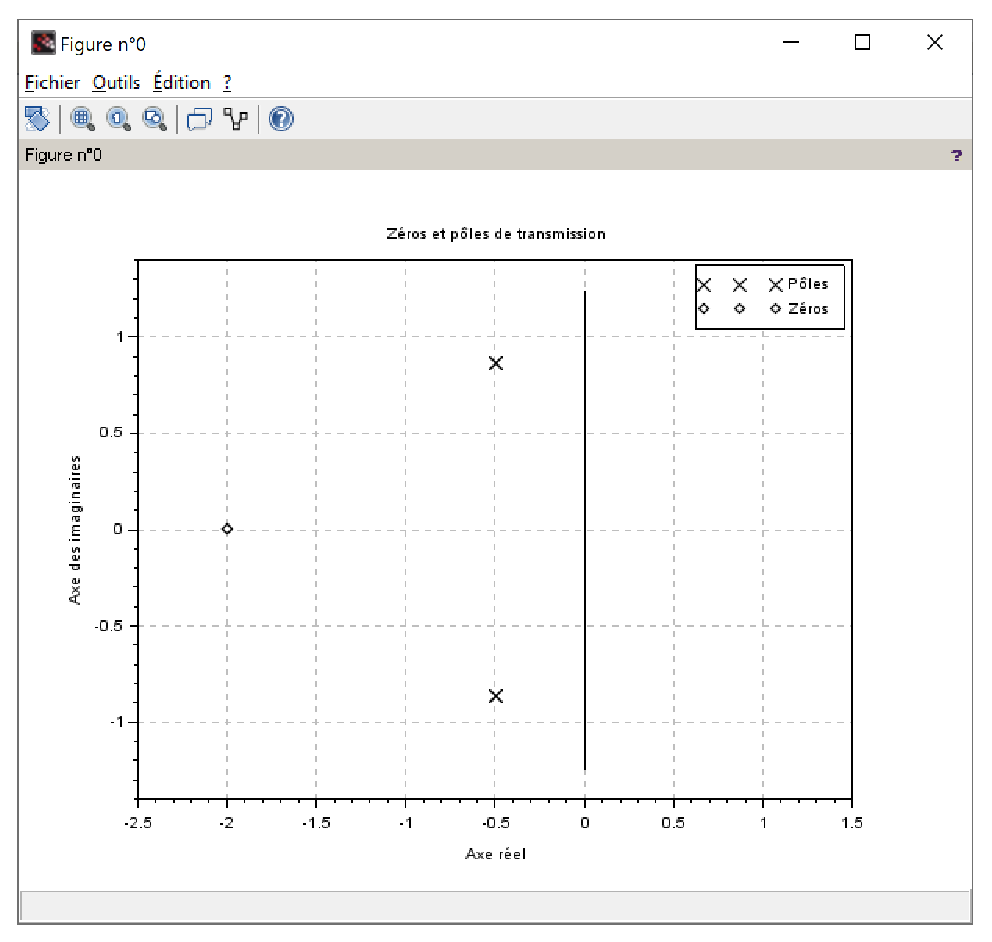
\includegraphics[width=0.8\textwidth]{fig/capture_SCILAB-plzr.eps}
\end{center}
%%%%%%%%%%%%%%%%%%%%%%%%%%%%%%%%%%%%%%%%%%%%%%%%%%%%%%%%%%%%%%%%%%%%%%%%%%%%%%%%
%%%%%%%%%%%%%%%%%%%%%%%%%%%%%%%%%%%%%%%%%%%%%%%%%%%%%%%%%%%%%%%%%%%%%%%%%%%%%%%%
\subsection{Asservissement}
%%%%%%%%%%%%%%%%%%%%%%%%%%%%%%%%%%%%%%%%%%%%%%%%%%%%%%%%%%%%%%%%%%%%%%%%%%%%%%%%
%%%%%%%%%%%%%%%%%%%%%%%%%%%%%%%%%%%%%%%%%%%%%%%%%%%%%%%%%%%%%%%%%%%%%%%%%%%%%%%%
\begin{doc}
%%%%%%%%%%%%%%%%%%%%%%%%%%%%%%%%%%%%%%%%%%%%%%%%%%%%%%%%%%%%%%%%%%%%%%%%%%%%%%%%
\paragraph{Fonction feedback (extrait de la doc officiel (en anglais): 
           help feedback)}
%%%%%%%%%%%%%%%%%%%%%%%%%%%%%%%%%%%%%%%%%%%%%%%%%%%%%%%%%%%%%%%%%%%%%%%%%%%%%%%%
\begin{itemize}
    \item Syntax :
    \begin{code}
\begin{verbatim}
Sl=Sl1/.Sl2
\end{verbatim}
    \end{code}
    \item Parameters :
    \begin{itemize}
        \item \verb?Sl1,Sl2?  linear systems (syslin list) in state-space or 
              transfer form, or ordinary gain matrices.
        \item \verb?Sl? linear system (syslin list) in state-space or 
              transfer form.
    \end{itemize}

    \item Description :

    \begin{itemize} 
        \item The feedback operation is denoted by /. (slashdot). 
        \item This command returns \verb?Sl=Sl1*(I+Sl2*Sl1)^-1?, i.e 
              the (negative) feedback of \verb?Sl1? and \verb?Sl2?. \verb?Sl? 
              is the transfer \verb?v -> y? for 
              \verb?y = Sl1 u?, \verb?u = v - Sl2 y?.
        \item The result is the same as \verb?Sl=LFT([0,I;I,-Sl2],Sl1)?.
        \item Caution: do not use with decimal point (e.g. \verb?1/.1? 
              is ambiguous!)
    \end{itemize}
\end{itemize}
\end{doc}

\paragraph{Exemple}
Imaginons que nous souhaitons déterminer
le système linéaire en boucle fermée à partir des systèmes de la chaîne directe $H(p)$
et la chaîne de retour $R(p)$ comme définit par le schéma-bloc suivant:
\begin{center}
    \tikzsetnextfilename{feedback-annexe_scilab-ext}
    \begin{tikzpicture}
    \bbr
\end{tikzpicture}

\end{center}
Avec cette opération \verb?feedback?, il est possible de déterminer la fonction de transfert 
en boucle fermée en une seule instruction.
\begin{code}
\begin{verbatim}
--> p=%s
--> H=syslin('c',1,1+p);
--> R=syslin('c',1,1+p);
--> HBF=H/.R
 HBF  = 
                 
       1 + s      
     -----------  
               2  
     2 + 2s + s 
\end{verbatim}
\end{code}

%\newpage
%%%%%%%%%%%%%%%%%%%%%%%%%%%%%%%%%%%%%%%%%%%%%%%%%%%%%%%%%%%%%%%%%%%%%%%%%%%%%%%%
%%%%%%%%%%%%%%%%%%%%%%%%%%%%%%%%%%%%%%%%%%%%%%%%%%%%%%%%%%%%%%%%%%%%%%%%%%%%%%%%
%%%%%%%%%%%%%%%%%%%%%%%%%%%%%%%%%%%%%%%%%%%%%%%%%%%%%%%%%%%%%%%%%%%%%%%%%%%%%%%%
\section{Scilab-Xcos}
%%%%%%%%%%%%%%%%%%%%%%%%%%%%%%%%%%%%%%%%%%%%%%%%%%%%%%%%%%%%%%%%%%%%%%%%%%%%%%%%
%%%%%%%%%%%%%%%%%%%%%%%%%%%%%%%%%%%%%%%%%%%%%%%%%%%%%%%%%%%%%%%%%%%%%%%%%%%%%%%%
%%%%%%%%%%%%%%%%%%%%%%%%%%%%%%%%%%%%%%%%%%%%%%%%%%%%%%%%%%%%%%%%%%%%%%%%%%%%%%%%
Nous présentons ici le module Xcos intégré à Scilab. Xcos inclut un 
éditeur graphique pour facilement représenté les schémas fonctionnels
en connectant des blocs entre eux. Cette présentation/tutoriel étant loin 
d'être complète, nous renvoyons le lecteur à la documentation officielle de Xcos
pour obtenir davantage de détails~\cite{steer2014scilab,premier,xcos}. 
%sur l'utilisation de ce module (notamment les références
%suivantes~\cite{steer2014scilab,premier,xcos}, sur lesquelles est basé le 
petit tuto suivant.)

%%%%%%%%%%%%%%%%%%%%%%%%%%%%%%%%%%%%%%%%%%%%%%%%%%%%%%%%%%%%%%%%%%%%%%%%%%%%%%%%
%%%%%%%%%%%%%%%%%%%%%%%%%%%%%%%%%%%%%%%%%%%%%%%%%%%%%%%%%%%%%%%%%%%%%%%%%%%%%%%%
\subsection{Lancer Xcos}
%%%%%%%%%%%%%%%%%%%%%%%%%%%%%%%%%%%%%%%%%%%%%%%%%%%%%%%%%%%%%%%%%%%%%%%%%%%%%%%%
%%%%%%%%%%%%%%%%%%%%%%%%%%%%%%%%%%%%%%%%%%%%%%%%%%%%%%%%%%%%%%%%%%%%%%%%%%%%%%%%
Après avoir lancé Scilab, éxécuter une des instructions suivantes :
\begin{itemize}
    \item Taper la commande \verb?xcos? dans la console;
    \item Cliquer sur l'icône : \raisebox{-\mydepth}{\fbox{
          
\includegraphics[height=\myheight]{fig/xcos.eps}}}
    \item Menu $\rightarrow$ Applications $\rightarrow$ Xcos
\end{itemize}

Xcos ouvre par défaut le navigateur de palettes et une fenêtre d'édition. 
Pour construire le diagramme il suffit de faire glisser les blocs dans la 
fenêtre d'édition.

%%%%%%%%%%%%%%%%%%%%%%%%%%%%%%%%%%%%%%%%%%%%%%%%%%%%%%%%%%%%%%%%%%%%%%%%%%%%%%%%
%%%%%%%%%%%%%%%%%%%%%%%%%%%%%%%%%%%%%%%%%%%%%%%%%%%%%%%%%%%%%%%%%%%%%%%%%%%%%%%%
\subsection{Diagramme simple}
%%%%%%%%%%%%%%%%%%%%%%%%%%%%%%%%%%%%%%%%%%%%%%%%%%%%%%%%%%%%%%%%%%%%%%%%%%%%%%%%
%%%%%%%%%%%%%%%%%%%%%%%%%%%%%%%%%%%%%%%%%%%%%%%%%%%%%%%%%%%%%%%%%%%%%%%%%%%%%%%%

Le module inclut un grand nombre de blocs (c.f Navigateur de palettes).
Il est possible de construire des super-blocs qui incorpore d'autres blocs pour
faciliter la lecture d'un diagramme complexe. \newline
Nous allons créer un diagramme simple. Pour celà, placer les blocs suivants 
dans la fenêtre d'édition:

\begin{table}[!h]
    \centering
    \begin{tabular}{@{}P{4cm}P{6cm}P{4cm}@{}}
    \toprule
    Désignation   & Représentation & Sous-palette \\
    \midrule
    \'Echelon     & 
    \begin{minipage}{6cm}
    \centering
    
\includegraphics[width=0.25\linewidth]{fig/scilab05.eps}
    \end{minipage} &
    Sources / STEP\_FUNCTION \\
    \midrule
    Fonction de transfert continue     & 
    \begin{minipage}{6cm}
    \centering
    
\includegraphics[width=0.25\linewidth]{fig/scilab06.eps}
    \end{minipage} & 
    Systèmes à temps continu / CLR \\
    \midrule
    Horloge       & 
    \begin{minipage}{6cm}
    \centering
    
\includegraphics[width=0.2\linewidth]{fig/scilab07.eps}
    \end{minipage} & 
    Sources / Clock\_c \\
    \midrule
    Visualisation & 
    \begin{minipage}{6cm}
    \centering
    
\includegraphics[width=0.25\linewidth]{fig/scilab08.eps}
    \end{minipage} & 
    Sinks / CSCOPE \\
    \bottomrule
\end{tabular}
\end{table}

Connecter les blocs pour obtenir le schéma bloc Xcos de la 
figure~\ref{fig-simple}.

\begin{figure}
    \centering
    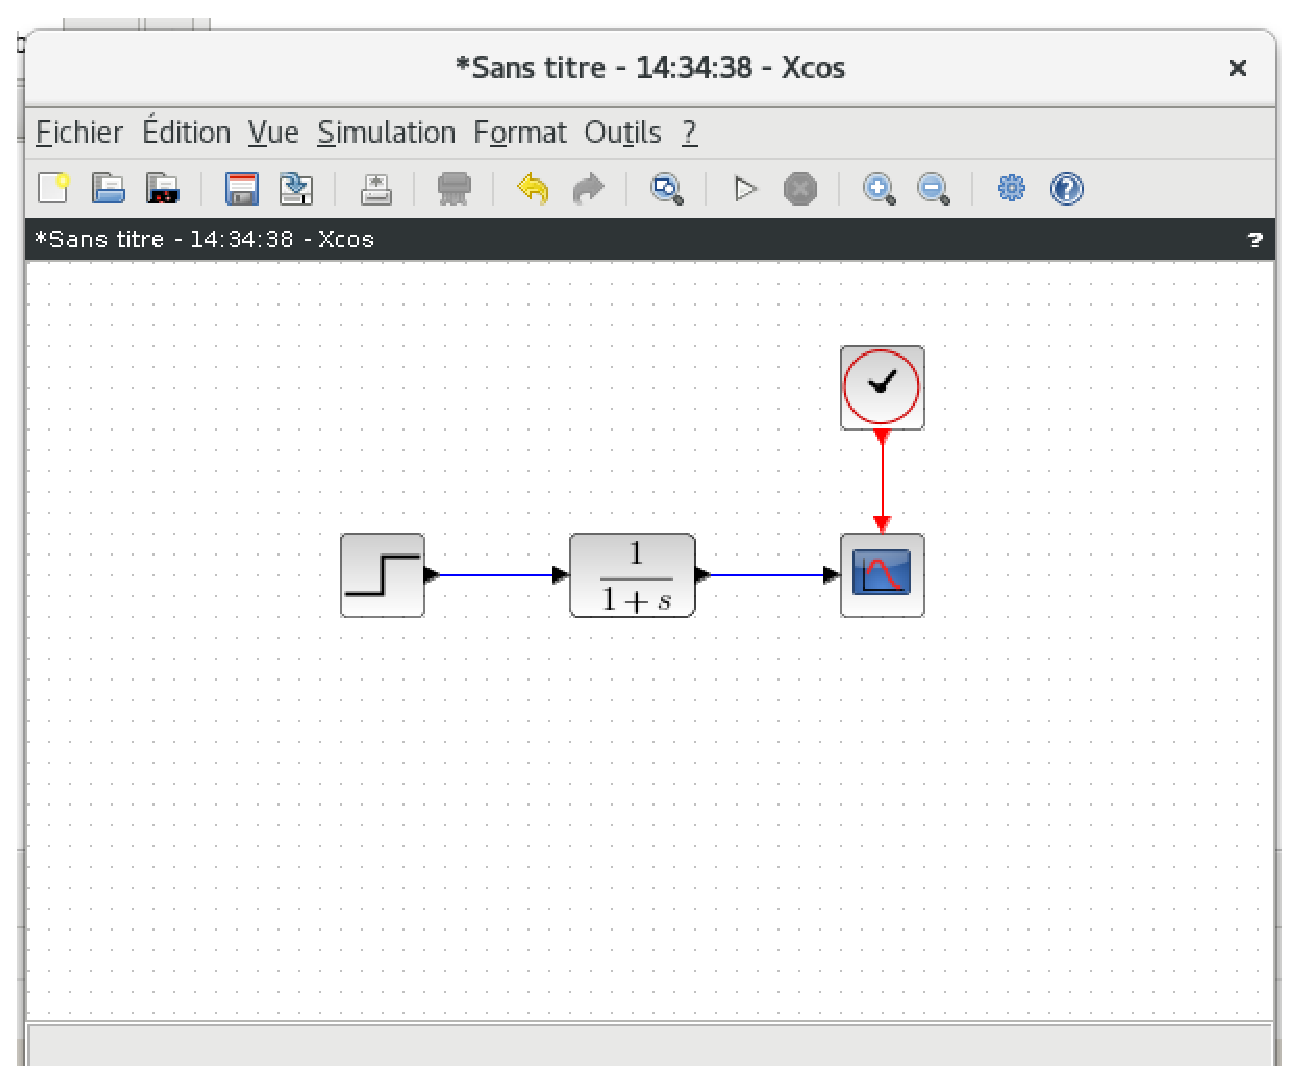
\includegraphics[width=0.5\textwidth]{fig/diagramme_simple.eps}
    \caption{Exemple de diagramme simple\label{fig-simple}}
\end{figure}

Il faut maintenant simuler et visualiser les résultats.  

%\newpage
%%%%%%%%%%%%%%%%%%%%%%%%%%%%%%%%%%%%%%%%%%%%%%%%%%%%%%%%%%%%%%%%%%%%%%%%%%%%%%%%
%%%%%%%%%%%%%%%%%%%%%%%%%%%%%%%%%%%%%%%%%%%%%%%%%%%%%%%%%%%%%%%%%%%%%%%%%%%%%%%%
\subsection{Simulation}
%%%%%%%%%%%%%%%%%%%%%%%%%%%%%%%%%%%%%%%%%%%%%%%%%%%%%%%%%%%%%%%%%%%%%%%%%%%%%%%%
%%%%%%%%%%%%%%%%%%%%%%%%%%%%%%%%%%%%%%%%%%%%%%%%%%%%%%%%%%%%%%%%%%%%%%%%%%%%%%%%
Pour lancer une simulation : cliquer sur l'icône : 
\raisebox{-\mydepth}{
    \fbox{
\includegraphics[height=\myheight]{fig/demarrage.eps}}
}

Pour arrêter une simulation : cliquer sur l'icône : 
\raisebox{-\mydepth}{
    \fbox{
\includegraphics[height=\myheight]{fig/stop.eps}}
}

Plusieurs paramètres peuvent être ajustés :
\begin{itemize}
    \item La durée de la simulation : Simulation $\rightarrow$ 
          Configurer $\rightarrow$ Temps d'intégration final
    \item La période d'échantillonage : Cliquer sur l'horloge.
    \item La fonction échelon  : Cliquer sur le bloc de la fonction échelon
    \item Les paramètres de la fonction de transfert : Cliquer sur le bloc CLR 
          (N'oubliez pas d'ajouter un contexte si vous utiliser des variables)
\end{itemize}

%%%%%%%%%%%%%%%%%%%%%%%%%%%%%%%%%%%%%%%%%%%%%%%%%%%%%%%%%%%%%%%%%%%%%%%%%%%%%%%%
%%%%%%%%%%%%%%%%%%%%%%%%%%%%%%%%%%%%%%%%%%%%%%%%%%%%%%%%%%%%%%%%%%%%%%%%%%%%%%%%
\subsection{Blocs \og To Workspace \fg~ou \og From Workspace\fg}
%%%%%%%%%%%%%%%%%%%%%%%%%%%%%%%%%%%%%%%%%%%%%%%%%%%%%%%%%%%%%%%%%%%%%%%%%%%%%%%%
%%%%%%%%%%%%%%%%%%%%%%%%%%%%%%%%%%%%%%%%%%%%%%%%%%%%%%%%%%%%%%%%%%%%%%%%%%%%%%%%
On utilisera les blocs particuliers dans le cas où l'on souhaite 
utiliser des données à partir de Scilab (\og From Workspace\fg) 
ou récupérer ces données après la simulation (\og To Workspace \fg).

\begin{figure}[!h]
    \centering
    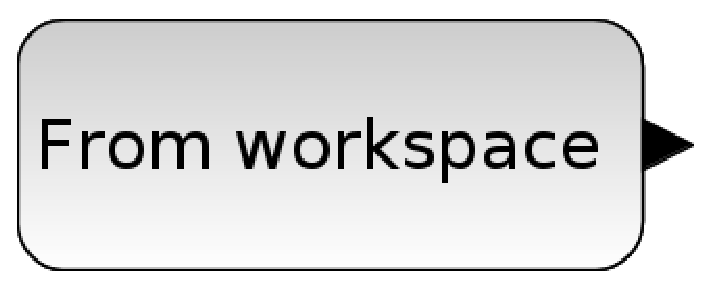
\includegraphics[width=0.25\textwidth]{fig/FROMWSB.eps}\hspace{3cm}
    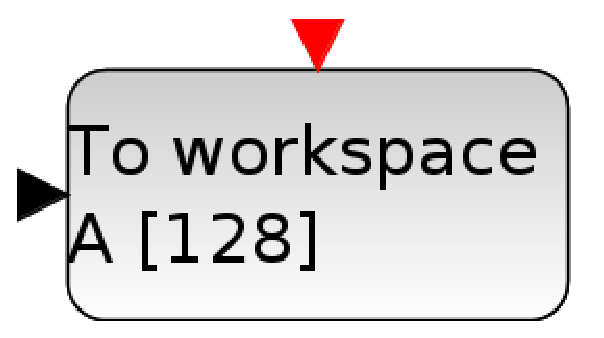
\includegraphics[width=0.25\textwidth]{fig/TOWS_c.eps}
    \caption{Blocs d'échange avec Scilab\label{fig-workspace}}
\end{figure}
%%%%%%%%%%%%%%%%%%%%%%%%%%%%%%%%%%%%%%%%%%%%%%%%%%%%%%%%%%%%%%%%%%%%%%%%%%%%%%%%
%%%%%%%%%%%%%%%%%%%%%%%%%%%%%%%%%%%%%%%%%%%%%%%%%%%%%%%%%%%%%%%%%%%%%%%%%%%%%%%%
%%%%%%%%%%%%%%%%%%%%%%%%%%%%%%%%%%%%%%%%%%%%%%%%%%%%%%%%%%%%%%%%%%%%%%%%%%%%%%%%
%%%%%%%%%%%%%%%%%%%%%%%%%%%%%%%%%%%%%%%%%%%%%%%%%%%%%%%%%%%%%%%%%%%%%%%%%%%%%%%%
%annexe_scilab.tex
